\section{Network Security}

\subsection{Network Segmentation}

\begin{definition}{Network Segmentation}\\
Network segmentation is the practice of dividing a computer network into smaller, isolated segments:
\begin{itemize}
    \item Increases operational performance by containing traffic
    \item Limits damage from cyber attacks to specific segments
    \item Protects vulnerable devices by isolating them
    \item Reduces the scope of compliance requirements
    \item Protects against insider threats
\end{itemize}
\end{definition}

\begin{concept}{Typical Network Segments}\\
Common network segments in organizations include:
\begin{itemize}
    \item \textbf{DMZ (Demilitarized Zone)} - Hosts public-facing services
    \item \textbf{Server Network} - Hosts internal servers and applications
    \item \textbf{Client Network} - Hosts employee workstations
    \item \textbf{Guest Network} - Hosts visitor devices with limited access
    \item \textbf{IoT Network} - Hosts Internet of Things devices
    \item \textbf{Industrial Network} - Hosts industrial control systems
    \item \textbf{Admin Network} - Hosts administrative systems and tools
\end{itemize}
\end{concept}

\subsection{Packet Filtering Firewalls}

\begin{definition}{Packet Filtering Firewalls}\\
Packet filtering firewalls control traffic flow between network segments:
\begin{itemize}
    \item Examine packet headers to make filtering decisions
    \item Apply rules based on source/destination addresses, ports, and protocols
    \item Operate at the network and transport layers of the OSI model
    \item Form the foundation of network security architecture
\end{itemize}
\end{definition}

\begin{concept}{Firewall Rule Management}\\
Effective firewall management requires structured processes:
\begin{itemize}
    \item \textbf{New Request} - Submission, approval, design, testing, deployment, validation
    \item \textbf{Operation} - Monitoring, audits, reports
    \item \textbf{Recertification} - Regular review of existing rules
    \item \textbf{Decommissioning} - Removal of unnecessary rules
\end{itemize}
Without proper management processes, firewall rule sets tend to grow uncontrolled and become difficult to understand.
\end{concept}

\begin{theorem}{Firewall Benefits and Limitations}\\
Firewalls provide significant security benefits but have limitations:
\begin{itemize}
    \item \textbf{Benefits}:
    \begin{itemize}
        \item Block unwanted traffic before it enters protected networks
        \item Centralize access control
        \item Hide internal network structure
    \end{itemize}
    \item \textbf{Limitations}:
    \begin{itemize}
        \item Primarily perimeter protection (assumes threats are external)
        \item Cannot prevent internal threats
        \item Basic packet filtering cannot detect application-layer attacks
        \item Cannot protect against allowed protocols misuse
    \end{itemize}
\end{itemize}
\end{theorem}

\subsection{Next Generation Firewalls (NGFW)}

\begin{definition}{Next Generation Firewalls}\\
NGFWs extend traditional firewall capabilities with additional features:
\begin{itemize}
    \item \textbf{Deep Packet Inspection} - Examines packet contents, not just headers
    \item \textbf{Application Awareness} - Identifies and controls traffic by application
    \item \textbf{Intrusion Prevention} - Detects and blocks network attacks
    \item \textbf{Antivirus/Anti-malware} - Scans traffic for malicious content
    \item \textbf{Sandboxing} - Executes suspicious files in isolated environments
    \item \textbf{Threat Intelligence} - Incorporates external information about threats
\end{itemize}
\end{definition}

\subsection{Microsegmentation}

\begin{definition}{Microsegmentation}\\
Microsegmentation takes network segmentation to a more granular level:
\begin{itemize}
    \item Segments as small as individual workloads or applications
    \item Implemented through network virtualization or host-based firewalls
    \item Limits lateral movement within a traditional network segment
    \item Reduces the attack surface and blast radius
    \item Balances security with management complexity
\end{itemize}
\end{definition}

\begin{concept}{Zero Trust Architecture}\\
Zero Trust is a security model that assumes no implicit trust within or outside the network:
\begin{itemize}
    \item \textbf{Core Principles}:
    \begin{itemize}
        \item Verify explicitly - Always authenticate and authorize
        \item Use least privilege access - Provide minimal necessary access
        \item Assume breach - Operate as if attackers are already present
    \end{itemize}
    \item \textbf{Components}:
    \begin{itemize}
        \item Policy Enforcement Point (PEP) - Enforces access decisions
        \item Policy Decision Point (PDP) - Makes access decisions
        \item Policy Administration Point (PAP) - Manages policies
    \end{itemize}
\end{itemize}
\end{concept}

\begin{theorem}{Zero Trust Challenges}\\
While Zero Trust offers significant security benefits, it presents several challenges:
\begin{itemize}
    \item Single points of failure in policy enforcement
    \item Potential for accidental or malicious misconfigurations
    \item Vulnerability to denial-of-service attacks
    \item Difficulties with encrypted traffic visibility
    \item Lack of protection against credential theft
\end{itemize}
\end{theorem}

\subsection{Host-Based Security}

\begin{definition}{Host-Based Firewalls}\\
Host-based firewalls provide an additional layer of protection:
\begin{itemize}
    \item Operate directly on individual devices
    \item Protect against threats that bypass network firewalls
    \item Filter traffic based on local policies
    \item Examples include Windows Defender Firewall, Linux nftables, and macOS firewall
\end{itemize}
\end{definition}

\begin{concept}{Endpoint Detection and Response (EDR)}\\
EDR systems combine several capabilities to secure endpoints:
\begin{itemize}
    \item \textbf{Monitoring}:
    \begin{itemize}
        \item Anomaly detection
        \item Vulnerability scanning
        \item Integrity checks
    \end{itemize}
    \item \textbf{Protection}:
    \begin{itemize}
        \item Host-based firewall
        \item Antivirus/anti-malware
        \item Application control
    \end{itemize}
    \item \textbf{Investigation and Response}:
    \begin{itemize}
        \item Device isolation
        \item User session termination
        \item Change rollback
        \item Evidence collection
    \end{itemize}
\end{itemize}
\end{concept}

\subsection{Application Protection}

\begin{definition}{Web Application Firewalls (WAF)}\\
WAFs protect web applications from attacks:
\begin{itemize}
    \item Examine HTTP/HTTPS traffic at the application layer
    \item Protect against OWASP Top 10 vulnerabilities:
    \begin{itemize}
        \item Cross-Site Scripting (XSS)
        \item SQL Injection
        \item Cross-Site Request Forgery (CSRF)
        \item Others
    \end{itemize}
    \item Require TLS termination to inspect encrypted traffic
    \item Deploy in front of web servers
\end{itemize}
\end{definition}

\subsection{Secure Web Gateways and Cloud Security}

\begin{definition}{Secure Web Gateway (SWG)}\\
SWGs protect users from web-based threats:
\begin{itemize}
    \item URL filtering to block malicious sites
    \item Data Loss Prevention (DLP) to prevent sensitive data exfiltration
    \item TLS inspection to examine encrypted traffic
    \item User and application control
\end{itemize}
\end{definition}

\begin{concept}{Cloud Access Security Broker (CASB)}\\
CASBs provide security controls for cloud services:
\begin{itemize}
    \item \textbf{Shadow IT discovery} - Identify unauthorized cloud service usage
    \item \textbf{Cloud usage control} - Set access rights to cloud services
    \item \textbf{Data leakage prevention} - Control data sharing in cloud services
    \item \textbf{Anomaly detection} - Alert on unusual behavior patterns
    \item \textbf{Implementation methods}:
    \begin{itemize}
        \item API scanning - Directly interfaces with cloud providers
        \item Forward proxy - Controls outbound access to cloud services
        \item Reverse proxy - Intermediates between users and cloud services
    \end{itemize}
\end{itemize}
\end{concept}

\subsection{Network Detection and Response}

\begin{definition}{Network Detection and Response (NDR)}\\
NDR systems monitor network traffic to detect and respond to threats:
\begin{itemize}
    \item Establish baseline network behavior
    \item Detect anomalies that may indicate attacks
    \item Analyze potential incidents to identify true positives
    \item Automatically respond to confirmed threats
\end{itemize}
\end{definition}

\begin{concept}{Security Information and Event Management (SIEM)}\\
SIEM systems collect and analyze security events:
\begin{itemize}
    \item Aggregate logs from multiple sources
    \item Correlate events to identify attack patterns
    \item Provide a centralized dashboard for security monitoring
    \item Generate reports for compliance and security analysis
\end{itemize}
\end{concept}

\begin{concept}{Security Orchestration\, Automation and Response (SOAR)}\\
SOAR platforms extend SIEM capabilities:
\begin{itemize}
    \item Automate security response with playbooks
    \item Integrate with multiple security tools
    \item Orchestrate complex security workflows
    \item Enhance incident response with automation
\end{itemize}
\end{concept}

\subsection{Linux Firewall with nftables}

\begin{definition}{nftables Framework}\\
nftables is a packet classification and filtering framework in Linux:
\begin{itemize}
    \item Replaces the legacy iptables framework
    \item Part of the Linux kernel since version 2.4
    \item Provides packet filtering, network address translation, and packet mangling
    \item Configured using the nft command-line tool
\end{itemize}
\end{definition}

\begin{concept}{nftables Architecture}\\
nftables uses a hierarchical structure:
\begin{itemize}
    \item \textbf{Tables} - Group chains for a specific packet type (address family)
    \item \textbf{Chains} - Group rules and attach to hooks in the network stack
    \item \textbf{Rules} - Define matching criteria and actions for packets
    \item \textbf{Expressions} - Match packet properties (addresses, ports, etc.)
    \item \textbf{Actions} - Determine what happens to matching packets (accept, drop, reject, etc.)
\end{itemize}
\end{concept}

\begin{code}{Basic nftables Commands}\\
\begin{lstlisting}[language=bash, style=basesmol]
# Create a table
nft add table inet filter

# Create a chain in the table
nft add chain inet filter input { type filter hook input priority 0 \; policy drop \; }

# Add a rule to the chain
nft add rule inet filter input tcp dport 22 accept

# List the ruleset
nft list ruleset

# Delete a rule (using its handle)
nft delete rule inet filter input handle 4

# Flush a table (delete all chains and rules)
nft flush table inet filter
\end{lstlisting}
\end{code}

\begin{KR}{Creating a Basic Firewall with nftables}\\
\paragraph{Setup Tables and Chains}
\begin{itemize}
    \item Create table for IPv4 and IPv6 traffic
    \item Create input, forward, and output chains
    \item Set default policies (usually drop for input and forward, accept for output)
\end{itemize}

\paragraph{Add Basic Rules}
\begin{itemize}
    \item Allow established and related connections
    \item Allow loopback traffic
    \item Allow specific services (SSH, HTTP, etc.)
    \item Allow ICMP/ICMPv6 for diagnostics
\end{itemize}

\paragraph{Add Protection Rules}
\begin{itemize}
    \item Drop invalid packets
    \item Implement rate limiting for certain traffic
    \item Log suspicious traffic
\end{itemize}

\paragraph{Test and Save}
\begin{itemize}
    \item Test connectivity from various sources
    \item Save ruleset to persist across reboots
    \item Implement monitoring to detect issues
\end{itemize}
\end{KR}

\subsection{Port Scanning}

\begin{definition}{Port Scanning}\\
Port scanning is a technique to discover available services on a network:
\begin{itemize}
    \item Identifies open ports on target systems
    \item Helps determine running services and potential vulnerabilities
    \item Used by both attackers for reconnaissance and administrators for security testing
    \item Most commonly performed using tools like nmap
\end{itemize}
\end{definition}

\begin{examplecode}{Basic Port Scanning with nmap}\\
\begin{lstlisting}[language=bash, style=basesmol]
# Scan a single host for common ports
nmap 192.168.1.1

# Scan specific ports
nmap -p 22,80,443 192.168.1.1

# Scan a range of ports
nmap -p 1-1000 192.168.1.1

# Scan an entire subnet
nmap 192.168.1.0/24

# Perform a service version scan
nmap -sV 192.168.1.1

# Perform an OS detection scan
nmap -O 192.168.1.1

# Perform a comprehensive scan
nmap -A 192.168.1.1

# Scan without ping (useful if ICMP is blocked)
nmap -Pn 192.168.1.1
\end{lstlisting}
\end{examplecode}

\begin{example}
A security administrator needs to verify that a newly implemented firewall is correctly filtering traffic between network segments. They use nmap to scan hosts in the protected segment from an external testing machine:

\texttt{nmap -Pn -sT -p 1-1024 10.0.1.10}

The scan reveals that only ports 80 (HTTP) and 443 (HTTPS) are accessible, while all other ports show as "filtered," indicating that the firewall is properly blocking the traffic. Additional scans from authorized internal segments confirm that administrative ports like 22 (SSH) are only accessible from the management network.
\end{example}

\section{Firewalls}

\subsection{Firewall basics}

\begin{definition}{Firewall}\\
    A firewall is a device that sits between two or more networks to control the packet flow between them. Based on the security policy one or more firewalls are installed and configured.
\end{definition}

\begin{concept}{Firewall Capabilities}\\
    A firewall can
    \begin{itemize}
        \item Control access from internal network to the Internet and vice versa
        \item Block malicious incoming web traffic
    \end{itemize}
\end{concept}

\subsection{Packet-filtering firewall (Network Layer)}

\begin{definition}{Packet-filtering Firewall}\\
    \begin{itemize}
        \item Using rules, that decide whether to forward packets
        \item Inspect headers of network and transport layer protocols
        \item \textbf{Pro:} Very fast as they only check layer 3 and 4 protocol headers
        \item \textbf{Limitation:} Only control who is allowed to talk to whom
    \end{itemize}
\end{definition}

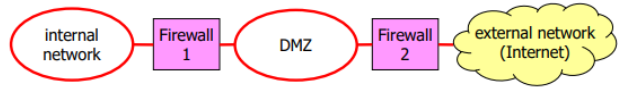
\includegraphics[width=\linewidth]{packet_filtering_firewall.png}

\subsection{Stateless firewall}

\begin{concept}{Stateless Firewall}\\
    \begin{itemize}
        \item Both directions need to be configured
        \begin{itemize}
            \item Every IP packet is handled completely isolated from all others
            \item Firewall does not keep track of ongoing communications
        \end{itemize}
        \item More open than needed: Replies from a server are allowed without a previous request from a client
        \item Limited support for complex protocols
    \end{itemize}

    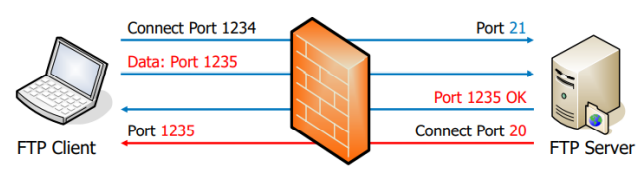
\includegraphics[width=\linewidth]{stateless_firewall.png}
\end{concept}

\subsection{Stateful firewall}

\begin{definition}{Stateful Firewall}\\
    Checks individual packets, tracks communication relationships, and maintains state information.
    \begin{itemize}
        \item Today standard
        \item Easier to configure (fewer rules)
        \item Return traffic is only allowed on demand
        \item Allows support for complex protocols
        \item A packet can be in one of four states: New, Established, Related, Invalid
    \end{itemize}
\end{definition}


\subsection{Application layer firewall (Application Layer)}

\begin{definition}{Application Layer Firewall}\\
    \begin{itemize}
        \item Split end-to-end communications
        \item Inspect application layer data
        \item \textbf{Pro:} Allows deep inspection of all data exchanged
        \item \textbf{Limitation:} Relatively slow, limitations with encrypted data
    \end{itemize}
\end{definition}

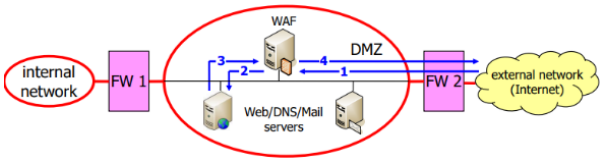
\includegraphics[width=\linewidth]{application_layer_firewall.png}

\subsection{Benefits and Limitations}

\begin{remark}
    Firewalls are only useful against attackers outside the internal network.
\end{remark}

\subsection{Linux netfilter/nftables}

\begin{definition}{netfilter/nftables}\\
    netfilter is a mechanism that allows to access the packets in the network stack to analyze, modify, extract, and delete them.
    \begin{itemize}
        \item Hooks that are called at different points during packet processing
    \end{itemize}
    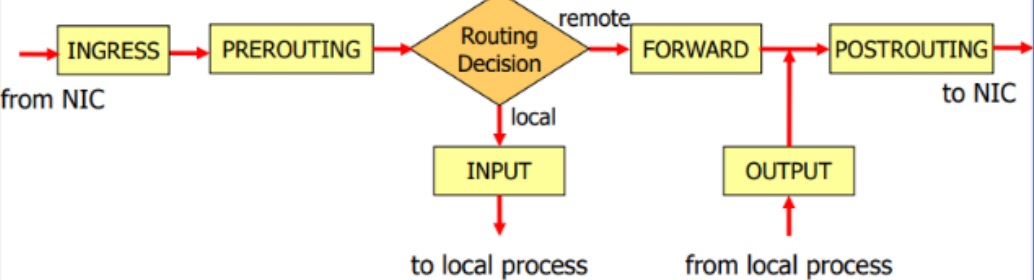
\includegraphics[width=\linewidth]{netfilter.png}
    
    nftables is a packet classification and mangling framework that runs on rulesets that are applied to the packets
    \begin{itemize}
        \item \textbf{Table} Container for specific type of package
        \item \textbf{Chain} Container with rules for a specific hook
        \item \textbf{Hook} Called at different points of processing
        \item \textbf{Priority} Lowest priority first until rule is accepted
        \item \textbf{Policy} Default behaviour
        \item \textbf{Rule} Classification + Action
        \item \textbf{Classification} What packets does a rule apply to
        \item \textbf{Action} What to do with the packet
    \end{itemize}
    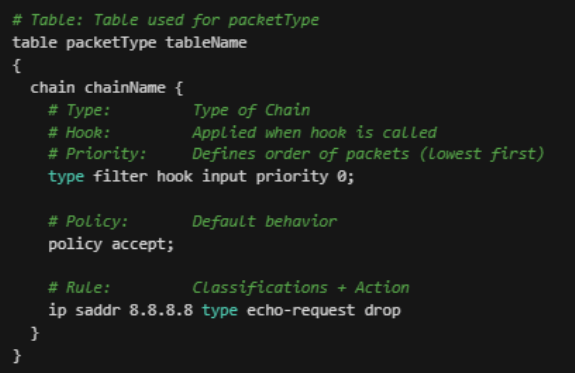
\includegraphics[width=\linewidth]{nftables.png}
\end{definition}



\subsection{Nftables Examples}

\begin{examplecode}{nftables Rules}\\
\begin{lstlisting}[language=bash, style=basesmol]
# Drop all packets going to IPv4 address 8.8.8.8
ip daddr 8.8.8.8 drop

# Accept all packets coming on interface eth2
iifname eth2 accept

# Accept all IPv6 packets carrying TCP
ip6 nexthdr tcp accept
\end{lstlisting}
\end{examplecode}

\subsection{Port scanning}

\begin{definition}{Port Scanning}\\
    Technique to determine the services that run on a host.
    \begin{itemize}
        \item Useful for attackers and system admins
        \item Port scanners...
        \begin{itemize}
            \item Check if the host is available by pinging it
            \item Establish TCP connections to the ports
        \end{itemize}
        \item Nmap: Most popular port scanner
        \item TCP scan of port 80 of www.zhaw.ch: \texttt{nmap -p80 www.zhaw.ch}
    \end{itemize}
\end{definition}